%+TITLE: Oscilador armónico y límite continuo
%+DESCRIPTION: Repaso del oscilador armónico, tomamos el límite continuo, y obtenemos nuestra primera teoría de campos: Ondas de sonido.
\documentclass[11pt,a4paper]{article}

\usepackage[utf8]{inputenc}
\usepackage[T1]{fontenc}
\usepackage[spanish,es-nodecimaldot]{babel}
\usepackage{lmodern}
\usepackage{amsmath,amssymb,mathtools}
\usepackage{graphicx}
\usepackage{xcolor}
\usepackage{geometry}
\usepackage{enumitem}
\usepackage{microtype}

\geometry{margin=2.3cm}
\setlength{\parindent}{0pt}
\setlength{\parskip}{0.65em}
\setlist[itemize]{leftmargin=1.6em,itemsep=0.25em,topsep=0.25em}

\definecolor{title-red}{RGB}{165,25,20}
\definecolor{concept-green}{RGB}{20,125,45}
\newcommand{\concept}[1]{\textcolor{concept-green}{#1}}

\newcommand{\ket}[1]{\left|#1\right\rangle}
\newcommand{\bra}[1]{\left\langle#1\right|}
\newcommand{\braket}[2]{\left\langle #1\middle|#2\right\rangle}
\newcommand{\hc}{\mathrm{h.c.}}
\newcommand{\Tr}{\operatorname{Tr}}
\newcommand{\Diffs}{\mathrm{Diffs}}

\begin{document}

Alguien dijo que la física es el estudio de aquellos fenómenos naturales que se reducen al oscilador armónico.

El lagrangiano del oscilador armónico es
\[
  L=\frac12 m\dot x^2-\frac12 m\omega^2x^2.
\]
La ecuación de Euler--Lagrange es
\[
  m\ddot x+m\omega^2x=0
  \qquad\Longrightarrow\qquad
  \ddot x+\omega^2x=0.
\]

Para resolverla usamos $e^{i\omega t}$. Note que
\[
  \frac{d}{dt}e^{i\omega t}=i\omega e^{i\omega t},
  \qquad
  \frac{d^2}{dt^2}e^{i\omega t}=-\omega^2e^{i\omega t}.
\]
La solución general es
\[
  x=\alpha e^{i\omega t}+\beta e^{-i\omega t},
\]
donde $\alpha$ y $\beta$ son números complejos.

Pero $x$ es una variable real, $x^*=x$, e imponiendo esto obtenemos
$\beta=\alpha^*$:
\[
  x=\alpha e^{i\omega t}+\alpha^*e^{-i\omega t}.
\]

Podemos conectarlo con la solución ``usual'' haciendo
\[
  e^{i\omega t}=\cos\omega t+i\sin\omega t.
\]
Entonces,
\begin{align*}
  x
  &=(\alpha+\alpha^*)\cos\omega t
    +i(\alpha-\alpha^*)\sin\omega t\\
  &=(2\operatorname{Re}\alpha)\cos\omega t
    -(2\operatorname{Im}\alpha)\sin\omega t.
\end{align*}

Ahora complicamos un poco estudiando dos osciladores acoplados.

\begin{figure}
  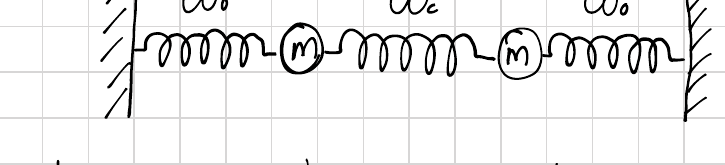
\includegraphics[width=0.72\textwidth]{figures/osciladores_acoplados.png}

  \caption{Dos masas acopladas por resortes de frecuencias
  $\omega_0$, $\omega_c$, $\omega_0$.}
\end{figure}

Nuestras coordenadas generalizadas son los desplazamientos de las masas respecto a la posición de equilibrio, $q_1,q_2$.

La energía potencial es
\[
  V(q_1,q_2)
  =\frac12m\omega_c^2(q_1-q_2)^2
   +\frac12m\omega_0^2q_1^2
   +\frac12m\omega_0^2q_2^2.
\]
El lagrangiano es
\[
  L
  =\frac12m\dot q_1^2+\frac12m\dot q_2^2
   -\frac12m\omega_c^2(q_1-q_2)^2
   -\frac12m\omega_0^2q_1^2
   -\frac12m\omega_0^2q_2^2.
\]
Las ecuaciones de movimiento son
\begin{align*}
  m\ddot q_1+m\omega_c^2(q_1-q_2)+m\omega_0^2q_1&=0,\\
  m\ddot q_2+m\omega_c^2(q_2-q_1)+m\omega_0^2q_2&=0.
\end{align*}

Demos un paso más. Consideremos una cadena infinita de osciladores armónicos acoplados.

\begin{figure}
  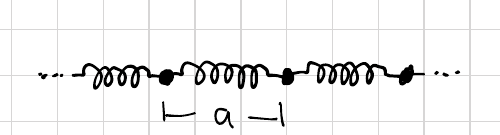
\includegraphics[width=0.55\textwidth]{figures/cadena_osciladores.png}

  \caption{Cadena infinita de osciladores separados una distancia $a$.}
\end{figure}

Su lagrangiano es
\[
  L
  =\frac12m\sum_{i=-\infty}^{\infty}\dot q_i^2
   -\frac12m\omega^2\sum_{i=-\infty}^{\infty}(q_{i+1}-q_i)^2.
\]
Las ecuaciones de movimiento son una para cada $q_i$:
\[
  \ddot q_i
  +\omega^2(q_i-q_{i+1})
  +\omega^2(q_i-q_{i-1})=0.
\]

Ahora queremos dar el paso de un sistema discreto a un sistema continuo. Esto nos dará nuestra primera teoría de campo. Para eso, llamamos $a$ a la separación en equilibrio. Tomaremos el límite $a\to0$, pero también $m\to0$ tal que $m/a$ permanece fijo.

Así mismo, las coordenadas generalizadas las tomamos como funciones de la posición del oscilador,
\[
  q_i\longrightarrow q(ia)=q(x).
\]
Esta función $q(x)$ representa el desplazamiento de un oscilador cuya posición de equilibrio es $x$.

Tomemos ese límite en el lagrangiano:
\begin{align*}
  \lim_{a\to0}L
  &=\lim_{a\to0}\sum_{i=-\infty}^{\infty}a
    \left[
      \frac12\left(\frac{m}{a}\right)\dot q^2(x)
      -\frac12am\omega^2
      \left(\frac{q(x)-q(x-a)}{a}\right)^2
    \right]\\
  &=\int_{-\infty}^{\infty}dx\,
    \left[
      \frac12\lambda\dot q^2(x)
      -\frac12Y\left(\frac{\partial q}{\partial x}\right)^2
    \right]\\
  &\equiv\int_{-\infty}^{\infty}dx\,
    \mathcal L\left(
      q(x,t),\dot q(x,t),\frac{\partial q(x,t)}{\partial x}
    \right),
\end{align*}
donde hemos definido
\[
  Y=\lim_{a\to0}am\omega^2,
\]
asumiendo que $\omega\to\infty$ tal que $a\omega$ es constante.

Tomemos también el límite en la ecuación de movimiento:
\[
  0=\lim_{a\to0}\left[
    \ddot q(x)
    +a\omega^2\left(
      \frac{q(x)-q(x-a)}{a}
      -\frac{q(x+a)-q(x)}{a}
    \right)
  \right].
\]

Para simplificar esto expandimos en serie de Taylor:
\begin{align*}
  q(x+a)
  &=q(x)+\frac{\partial q}{\partial x}(x)a
    +\frac12\frac{\partial^2q}{\partial x^2}(x)a^2
    +\mathcal O(a^3),\\
  q(x-a)
  &=q(x)-\frac{\partial q}{\partial x}(x)a
    +\frac12\frac{\partial^2q}{\partial x^2}(x)a^2
    +\mathcal O(a^3).
\end{align*}
Entonces,
\begin{align*}
  &(q(x)-q(x-a))-(q(x+a)-q(x))\\
  &\quad=
  \left(
    \frac{\partial q}{\partial x}a
    -\frac12\frac{\partial^2q}{\partial x^2}a^2
  \right)
  -\left(
    \frac{\partial q}{\partial x}a
    +\frac12\frac{\partial^2q}{\partial x^2}a^2
  \right)
  =\frac{\partial^2q}{\partial x^2}a^2.
\end{align*}
Por tanto,
\[
  \frac{\partial^2q}{\partial t^2}
  -\frac{Y}{\lambda}\frac{\partial^2q}{\partial x^2}=0,
\]
que es la ecuación de onda de sonido en una barra.

También podemos obtener esta ecuación variando la acción
\[
  S[q]
  =\int_{t_i}^{t_f}dt\int_{-\infty}^{\infty}dx\,
  \mathcal L(q,\partial_tq,\partial_xq).
\]
A la función $q(t,x)$ le agregamos una variación $\delta q(t,x)$. Para fijar
condiciones de borde pedimos que
\[
  \delta q(t_i,x)=0,
  \qquad
  \delta q(t_f,x)=0.
\]
Pedimos como antes que $\delta S[q]=0$:
\begin{align*}
  \delta S
  &=\int_{t_i}^{t_f}dt\int_{-\infty}^{\infty}dx\,
    \Bigl(
      \mathcal L(q+\delta q,
      \partial_tq+\partial_t\delta q,
      \partial_xq+\partial_x\delta q)
      -\mathcal L(q,\partial_tq,\partial_xq)
    \Bigr)\\
  &=\int_{t_i}^{t_f}dt\int_{-\infty}^{\infty}dx\,
    \left(
      \frac{\partial\mathcal L}{\partial q}\delta q
      +\frac{\partial\mathcal L}{\partial(\partial_tq)}
        \partial_t\delta q
      +\frac{\partial\mathcal L}{\partial(\partial_xq)}
        \partial_x\delta q
    \right)\\
  &=\int_{t_i}^{t_f}dt\int_{-\infty}^{\infty}dx\,
    \left[
      \frac{\partial\mathcal L}{\partial q}
      -\partial_t\left(
        \frac{\partial\mathcal L}{\partial(\partial_tq)}
      \right)
      -\partial_x\left(
        \frac{\partial\mathcal L}{\partial(\partial_xq)}
      \right)
    \right]\delta q\\
  &\quad+
    \left[
      \int_{-\infty}^{\infty}dx\,
      \frac{\partial\mathcal L}{\partial(\partial_tq)}\delta q
    \right]_{t_i}^{t_f}
    +\left[
      \int_{t_i}^{t_f}dt\,
      \frac{\partial\mathcal L}{\partial(\partial_xq)}\delta q
    \right]_{-\infty}^{\infty}.
\end{align*}

Asumimos que el campo $q$ y sus derivadas tienden rápidamente a cero en $x\to\pm\infty$. Excitar ondas en el infinito requiere una energía o un tiempo infinitos. Así obtenemos las ecuaciones de Euler--Lagrange para el campo:
\[
  \frac{\partial\mathcal L}{\partial q}
  -\partial_t\left(
    \frac{\partial\mathcal L}{\partial(\partial_tq)}
  \right)
  -\partial_x\left(
    \frac{\partial\mathcal L}{\partial(\partial_xq)}
  \right)=0.
\]

Aplicándolas a nuestra densidad lagrangiana
\[
  \mathcal L
  =\frac12\lambda\dot q^2
   -\frac12Y(\partial_xq)^2,
\]
tenemos
\[
  \frac{\partial\mathcal L}{\partial q}=0,
  \qquad
  \frac{\partial\mathcal L}{\partial\dot q}=\lambda\dot q,
  \qquad
  \frac{\partial\mathcal L}{\partial(\partial_xq)}=-Y\partial_xq,
\]
y por tanto
\[
  \lambda\ddot q-Y\partial_x^2q=0.
\]

\end{document}
